\ifdefined\included
\else
\setcounter{chapter}{0}
\dominitoc
\faketableofcontents
\fi

\chapter{Evolution of Human-Aware Navigation}
\chaptermark{Evolution of Human-Aware Navigation}
\label{chap:1}
\minitoc

% In this chapter, a formal definition of human-aware robot navigation is provided, followed by a description of the challenges involved. Then a brief explanation of how these challenges are currently addressed is provided. Further, we present the necessary background that is required to understand this thesis and then move on to the presentation of our approach. Before starting with HAN, we introduce general motion planning and robot navigation.

Beginning with the topic of robot navigation, this chapter outlines the development of human-aware (robot) navigation (HAN). We briefly talk about navigation in the context of motion planning and explain the methodologies and tools for 2D navigation. Then we present the evolution of HAN over the years using the existing literature before presenting a small discussion on how HAN is closely associated with \acrshort{hri}. Further, we also present the chronological developments and contributions of our lab to this field. Next, we present the challenges faced by the researchers in this field and discuss how they were addressed in the literature. Finally, we present our approach to HAN along with the required mathematical background. In addition, we explain how the joint-action principles can be applied to the context of human-aware navigation.

\section{Motion Planning and Navigation}

We briefly introduce the motion planning problem and robot navigation in this section. We present a detailed explanation of navigation in 2D and the different components involved in it. Finally, we provide a brief overview of the \acrshort{ros} based 2D navigation stack for mobile robots.

\subsection{The Motion Planning Problem}
Motion planning has varied applications in several fields \cite{latombe1999motion}, but robotics remains the core field of development. The intention behind any motion planning problem in robotics (manipulation or navigation) is to plan a continuous motion sequence for a robot to reach the final goal configuration from its initial configuration in a given environment while avoiding collisions. Although motion planning can refer to either path planning or trajectory planning, in this thesis, we treat them as the two steps of the motion planning problem. The first step is path planning which generates a collision-free path from start to goal. In the second step, the generated path is used as a guide, and a feasible trajectory is planned to trace this path partly or entirely. Generally, a path is a sequence of configurations, whereas a trajectory is a sequence of configurations and time differences that satisfy all the kinodynamic constraints. 

\subsubsection{Path Planning}
% Motion planning has varied applications in several fields \cite{latombe1999motion}, but robotics remains the core filed of development. 
Path planning in robotics deals with the generation of a continuous path from an initial configuration of the robot to a final or goal configuration while avoiding obstacles in the given environment. Hence it requires the description of the environment (2D or 3D grids, maps etc.) and a goal position as inputs for the path planning.

\begin{figure}[h!]
    \centering
    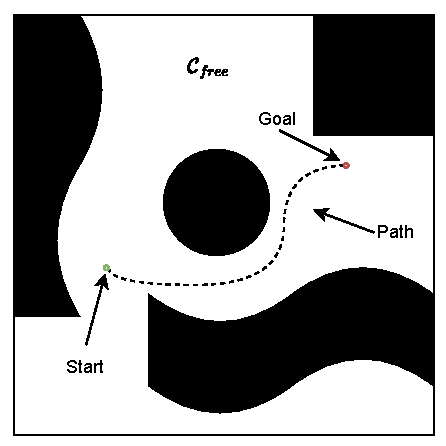
\includegraphics[width=0.45\columnwidth]{images/config_space.pdf}
    \caption{Motion Planning and Configuration Space}
    \label{fig:config_space}
\end{figure}

The configuration space, $\mathcal{C}$, for the path planning is the set of all possible configurations, and it depends on the type and degrees of freedom of the robot. For example, a mobile robot that can translate and rotate in 2D has a configuration space, $\mathcal{C} \in SE(2) = \mathbb{R}^2 \times SO(2)$, where $SE(2)$ is the special Euclidean group in 2D and $SO(2)$ is the special orthogonal group of 2D rotations. If the robot is a fixed base manipulator with $n$ degrees of freedom (or joints), then $\mathcal{C}$ is an $n$-dimensional vector. The subset of all configurations in $\mathcal{C}$ that is collision-free comprise the free space, $\mathcal{C}_{free}$. Hence, any path from start to goal should be within the $\mathcal{C}_{free}$ as shown in Fig.~\ref{fig:config_space}. 

\begin{figure}[h!]
    \centering
    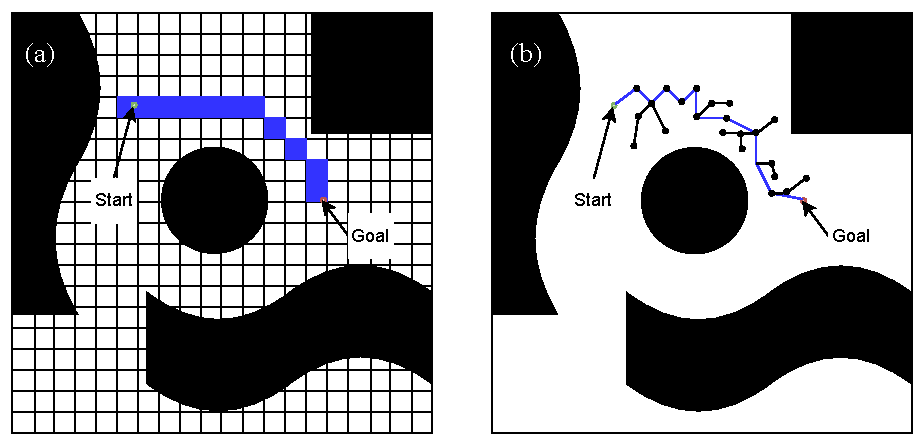
\includegraphics[width=0.9\columnwidth]{images/grid_vs_sampling.pdf}
    \caption{Path Planning. (a) Grid-based search (b) Sampling-based algorithm}
    \label{fig:grid_v_sample}
\end{figure}

Various methodologies can be employed to find a path, and the most famous ones are grid-based searches and sampling-based algorithms (Fig.~\ref{fig:grid_v_sample}). In grid-based methods, the entire configuration space is divided into small grids, and searching algorithms like A*~\cite{hart1968formal}, D*~\cite{stentz1997optimal} or Dijkstra are employed to search the connectivity from start to goal. A sample path generated using this method is shown in Fig.~\ref{fig:grid_v_sample} (a) (blue region). However, these methods suffer from the curse of dimensionality as the grid size becomes smaller and the configuration space (or map) becomes larger. Sampling-based algorithms like \acrshort{rrt}~\cite{lavalle1998rapidly} or \acrshort{prm}~\cite{kavraki1996probabilistic}, on the other hand, can handle high dimensional spaces better as their run-time is not exponentially dependent on the size or dimension of the configuration space, $\mathcal{C}$. These methodologies grow a connectivity map or tree from the starting position based on the points sampled in small regions. The sampled points are connected and added to the tree only if the connecting line segment is completely in $\mathcal{C}_{free}$. A path is found when the start and goal are connected by this tree, as shown in Fig.~\ref{fig:grid_v_sample} (b). The shortest connected path is shown in blue. These methods are probabilistically complete and will find a solution or a better solution as more time is spent searching but cannot verify if a solution exists or not. Other frequently used techniques involve artificial potential fields~\cite{vadakkepat2000evolutionary}, cell decomposition~\cite{garrido2006path} (for e.g. Voronoi regions), interval-based search etc. 


\subsubsection{Trajectory Planning}
Trajectory planning is used to generate the reference inputs for the robot's control system to execute the desired motion. Therefore, a trajectory is usually parameterised by time and can include the velocities and accelerations, apart from the configurations of the robot. The trajectory planning problem takes the path planned from the previous step as input, along with the kinodynamic constraints like the velocity, acceleration and kinematics of the robot to generate a continuous sequence of configurations and their associated time intervals. 

The planned trajectory can either be in the operating space (world frame) or the joint space (local frame) of the robot. If the motion of the robot has to follow certain geometric characteristics defined in the operating space (e.g. navigation), the trajectory planning is done in the operating space. To generate the reference control commands from this trajectory, kinematic inversion has to be performed, mapping the trajectory in the world frame to the desired controller or joint frames. As the degrees of freedom of a robot increase, this kinematic inversion for a densely populated trajectory becomes computationally expensive. Hence, trajectory planning is largely done in the joint space. For this, a set of waypoints are sampled from the planned path and mapped to the joint space using kinematic inversion. Then, trajectories are planned, such that all these waypoints are connected while satisfying the kinodynamic constraints. This can be done by interpolating between the points using a polynomial function or spline satisfying the constraints. Planning in joint spaces generally avoids the problems with redundant joints and singularities. However, the issue with such trajectory planning is that the robot might have some undesired configurations between these waypoints, and depending on the granularity of sampling, the number of these configurations might increase or decrease. 

No matter in which space the trajectories are planned, they should be continuous not only in terms of configurations but also in terms of velocity and acceleration to avoid jerks and vibrations of the robot while executing them. This means that the trajectory has to obey these additional constraints along with the kinodynamic constraints, and hence, it is often posed as an optimization problem. The most significant optimality criteria used for this are the minimum time, energy or jerk~\cite{gasparetto2015path}. One can employ any optimization technique like minimax~\cite{vathsal1977minimax}, genetic algorithms~\cite{tian2004effective}, multi-objective optimization~\cite{oleiwi2014multi}, unconstrained optimization~\cite{rosmann2013efficient}, or model predictive control~(\acrshort{mpc})~\cite{ardakani2015real} to solve this problem, depending on the requirements. Re-planning times for trajectory are usually large as it involves solving a complex optimization problem. Therefore, trajectory planning can either be global, covering the entire path, or local, covering only a small part of the path. For dynamic environments, local planning is employed so that the trajectory can be dynamically re-planned in real-time. Global trajectory planning is employed when the robot's operating space is constant and does not change over time. 

\subsubsection{Navigation and Manipulation}
Although both navigation and manipulation are motion planning problems and use similar algorithms, there are some basic differences. The navigation problem specifically deals with moving the entire robot from one place to another, whereas the manipulation problem deals with the motion of the end-effector and/or joints from the initial configuration to the goal configuration, while the base of the robot is assumed to be fixed. This thesis focuses only on the navigation problem, specifically mobile robot navigation on the ground using a 2D description of the world.

\subsection{Mobile Robot Navigation}
Mobile robot navigation is a well-studied field as it lays the foundation for autonomous vehicles and robots. Navigating in an unknown environment requires~\acrfull{slam}~\cite{thrun2007simultaneous} along with some kind of global positioning system (GPS) to guide the robot or vehicle to the goal. As global path planning cannot be done in such environments, robot navigation is largely handled by local motion planning and collision avoidance techniques. However, when it comes to the known environments with prior maps, the navigation problem can be split into two discrete parts, namely, localization and motion planning. The localization part of the problem continuously locates and tracks the position of the robot in either a static or dynamic environment~\cite{thrun2006probalistic}. Numerous methods can be employed for this like \acrshort{ekf} localization using landmarks, grid-based localization~\cite{thrun2006probalistic}, Monte-Carlo or Adaptive Monte-Carlo localization~\cite{fox2003adapting} using particles filters~\cite{fox2001particle}, vision-based localization~\cite{adorni2001vision} etc. In this thesis, we do not address the entire navigation problem and only focus on the motion planning part,
\begin{figure}[h!]
    \centering
    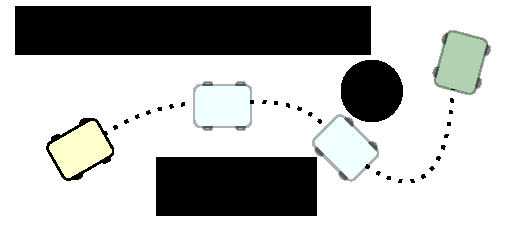
\includegraphics[width=0.9\columnwidth]{images/motion_planning_new.pdf}
    \caption{2D mobile robot Navigation from start (yellow) pose to goal (green) pose. The path planning problem has to plan the path and the intermediate poses (blue) that the robot needs to follow to reach the goal without colliding with the obstacles. The obstacles are marked in black. The trajectory planning then has to generate the control commands for the robot to follow this path.}
    \label{fig:navigation}
\end{figure}
which is usually referred to as `navigation planning'. As discussed in the previous section, given a goal configuration, in the case of 2D, a goal pose (position and orientation), the motion planning part (or navigation planning) has to solve the problem of the robot's motion from the start to the goal. Fig. \ref{fig:navigation} shows an example of such navigation planning avoiding the static obstacles in the environment. The path planned from the start pose to the goal pose of the robot in the free space, $\mathcal{C}_{free}$ is shown in this figure. The trajectory planner has to take this path as input and generate the control commands for the robot's base controller.

The maps for mobile robot navigation are usually represented as 2D occupancy-grids~\cite{thrun2006probalistic} as they are easy to acquire. The fundamental concept behind occupancy grids is to visualise the map as an evenly spaced grid of binary random variables. The occupancy grid based maps are built by updating the occupancy value of each grid using different kinds of range sensors like Sonars or \acrshort{lidar}s. Cameras and other sensors are also used in fusion with the range sensors to improve the accuracy of this estimation. However, all these methodologies assume that the robot knows its position and path in the map, which is generally provided by \acrshort{slam} techniques. Unless a blueprint of the environment is available, maps are built using \acrshort{slam} and Occupancy Grid mapping algorithms~\cite{thrun2006probalistic} and are used for path estimation. 

In such occupancy grids, search based path planning algorithms like modified A* \cite{warren1993fast} are much faster compared to sampling-based approaches like RRT-connect~\cite{kuffner2000rrt} or \acrshort{prm}~\cite{kavraki1996probabilistic}. Hence, in 2D navigation, path planning is done globally using grid-based search, which provides waypoints or a reference path for trajectory planning. The trajectory planning can be either local or global. Global trajectory planning will work in a setting where nothing moves or changes, and the environment remains in the same state as it was represented in a map. This is mostly true in the case of a manipulator, but for navigation, the environments usually change, and more obstacles like tables, chairs, beds etc., are added to the basic (static) environmental map. Hence, trajectory planning also requires obstacle information which is provided through the sensors. As the range of these sensors is limited, they can only provide information about the obstacles in a small region. Therefore, in a mobile robot navigation setting, the trajectory planning is mostly local, and it is interlinked with obstacle avoidance which modifies the trajectory of the robot to avoid collisions with obstacles found on its path. Some of the commonly used obstacle avoidance methods are \acrfull{dwa}~\cite{fox1997dynamic}, Elastic Bands~\cite{quinlan1993elastic} and artificial potential fields. Consequently, trajectory generation algorithms combined obstacle avoidance methods with their optimization scheme to produce online trajectories in real-time. However, these obstacle avoidance methods did not consider the velocity of the obstacles~\cite{cai2020mobile}, and hence, in the case of an environment with a lot of dynamic obstacles, the trajectory optimization had to be run at a high frequency which increased the computational cost and made online re-planning infeasible. 

Concurrently, collision avoidance strategies were developed for environments with a lot of dynamic obstacles or humans (treated as obstacles). These algorithms generate instantaneous velocities or control commands for the robot's base that ensure collision-free motion with fewer computational resources. Therefore, many works in literature employ collision avoidance techniques with global path planning for robot navigation in highly dynamic environments and crowds, which are sometimes called `reactive navigation' schemes. The trajectories were generated by accumulating a sequence of control commands provided by the collision avoidance strategies~\cite{prassler1999navigating}. These methodologies include velocity-obstacle based methods like \acrshort{rvo}~\cite{van2008reciprocal}, \acrshort{orca}~\cite{berg2011reciprocal} or \acrshort{calu}~\cite{hennes2012multi}, social force and reinforcement learning methods like \acrshort{cadrl}~\cite{chen2017decentralized}, \acrshort{sacadrl}~\cite{chen2017socially} or \acrshort{crl}~\cite{ciou2018composite}. This is still a very active research field as it helps to simulate and understand crowds. Although the collision avoidance methods can produce bounded velocities, the resultant trajectory is not guaranteed to be smooth in terms of acceleration and jerk. Consequently, researchers reverted to online trajectory planning, for example, \acrshort{mpc} and \acrfull{teb}, as computational power has significantly improved over this time. The main contribution of this thesis is an online trajectory planner based on timed elastic bands~\cite{rosmann2013efficient} while relying on grid-based path planning (Dijkstra or A*) to generate the path.

%%%%%%%%%%%%%%%navigation and localization%%%%%%%%%%%%%
% https://docs.ufpr.br/~danielsantos/ProbabilisticRobotics.pdf

% https://ieeexplore.ieee.org/stamp/stamp.jsp?arnumber=1638022&casa_token=AVdRjSBOau0AAAAA:qeaiZsQQatMpPRspPQm4TYjY87_q1e9CtAUrSsNfVvrMP1AHZQuaZrn0FGkeA6BrEExdYq_cugA

% https://ieeexplore.ieee.org/stamp/stamp.jsp?arnumber=8460519&casa_token=I-PESla6BaoAAAAA:BW_PXsnVSXss6jWDGMZyNrzYxx9gdr3sj5IbnQXIUzyooIbBNUOvaKTVzbW2litr-k2-o4bsQko

% https://ieeexplore.ieee.org/stamp/stamp.jsp?arnumber=8316333&casa_token=oSUKMnVKnAEAAAAA:1p1UiVL2SYsa54dgWfvnIsVgcphU6Wi6WfYQbjPqBKBA529pdvLQIkUJ4g1MlSxm3znUqlTyQNQ
%%%%%%%%%%%%%%%%%%%%%%%%%%%%%%%%%%%%%%%%%%%%%%%%%%%%%%%%%%

\subsection{2D Navigation Stack in ROS}
\acrfull{ros}~\cite{quigley2009ros} provides an environment to develop different tools for robotic platforms. It has several built-in packages and software bundles that make this development easier. Being an open-source platform, there are several custom packages and large community support to discuss and resolve issues. \acrshort{ros} readily supports motion planning and has official packages for navigation as well as manipulation. As the navigation planning system presented in this thesis is developed using the \acrshort{ros} Navigation Stack\footnote{\url{http://wiki.ros.org/navigation}}, we briefly present its features. The main package of this stack is \textit{\textbf{move\_base}} which provides the plugins to include new planners.

\textbf{Inputs}: Apart from the 2D navigation goal (position and orientation), the navigation stack takes as input the odometry information, the sensory data like laser or point cloud to obtain the real-time obstacle information and the static map data (as occupancy grid) for planning the path. It also requires the necessary transformation to connect the `\textit{map}' and the `\textit{base\_link}' of the robot, which usually is published by the localisation module. The navigation stack by default uses the \textbf{\textit{amcl}} package in \acrshort{ros} for robot localization. 

\textbf{Architecture}: The navigation stack has a `\textit{global planner}' that takes care of the path planning and a `\textit{local planner}' that deals with the trajectory planning. Both these planners are built as plugins and provide an easy way to use your own custom planners besides the existing ones. As it is built over \acrshort{ros}, the parameters and the planners can be updated easily using an `\textit{yaml}' configuration file. 

\textbf{Output}: It outputs the command velocity for the robot's base controller.

%%%%%%%%%%%Paper%%%%%%%%%%%%%%%%%
% https://www.researchgate.net/profile/Paolo-Boscariol/publication/282955967_Path_Planning_and_Trajectory_Planning_Algorithms_A_General_Overview/links/59ad4b580f7e9bdd115c2afb/Path-Planning-and-Trajectory-Planning-Algorithms-A-General-Overview.pdf
%%%%%%%%%%%Paper%%%%%%%%%%%%%%%%%

\section{Human-Aware Navigation}
\acrfull{han} deals with the navigation planning of the robot in human workspaces. Therefore, it has to take into account several factors while planning. We believe that HAN needs to integrate human expectations, social norms and situation analysis into its planning while taking care of other static and dynamic obstacles. It should try to lessen the discomfort and make the robot's motion more legible to the humans in the environment. 

In this section, we present various works related to HAN, distributed in four parts. We then proceed with a description of the research and evolution of HAN at our lab over the years and the proposed systems. Next, we briefly discuss how HAN is seen and used as a part of \acrshort{hri} before presenting the challenges faced by researchers in HAN. Finally, a short description of how these challenges are addressed is provided. 

\subsection{State-of-Art over the years}
We briefly present the works that are related to HAN in this section. This section is divided into four parts to show for ease of explanation and also to show how the number of works increased over time. We start with some early works and move on to the most recent literature. 

\subsubsection{The initial works: Before 2000}
Some of the early works in HAN were published before 2000. In the work by Tadokoro et al.~\cite{tadokoro1995motion}, a trajectory planning algorithm was presented that takes human motion prediction into account and plans the robot's motion. As the interest in the sector of service robots grew, new design philosophies and architectures were proposed like the ones by Kawamura et al.~\cite{kawamura1996design} and Wilkes et al.~\cite{wilkes1998toward}. During this period, one of the first robotic tour guides, RHINO~\cite{burgard1999museum}, was deployed in the “Deutsches Museum Bonn” for six days. According to the article by Burgard et al.~\cite{burgard1999experiences}, it had a success rate of over 99\%. Later, a second generation of the robotic tour guide, MINERVA~\cite{thrun1999minerva}, was deployed in the “Smithsonian’s National Museum of American History” for two weeks and gave 620 hours of tours. Both these robots used similar probabilistic architectures as mentioned in~\cite{burgard1999experiences} and~\cite{thrun2000probabilistic}. However, MINERVA had an additional interactive component and communicated its navigation intent through facial expressions and sounds~\cite{schulte1999spontaneous}. The work by~\cite{imai1999agent} presents a migration system with a computer generated agent that shifts from PC to the Pioneer I robot, which guides the people in their labs.

Robotic wheelchairs also have to address HAN along with the comfort of the person in the wheelchair. Yanco~\cite{yanco1998integrating} presented a list of the then-existing projects for robotic wheelchairs and proposed a wheelchair for indoor navigation~\cite{yanco1998wheelesley}. In parallel, Prassler et al.~\cite{prassler1999navigating} deployed their robotic wheelchair, MAid~\cite{prassler1998maid}, in a railway station during rush hour and through crowds to evaluate their navigation system. They used temporal maps with decaying observations over the grid for path planning and velocity-obstacle based evasive manoeuvres.
 
\subsubsection{The early 2000's: 2000-2006}
The number of works in the field started to rise over these years with an increased focus on robots for human-aid. Boy et al.~\cite{boy2002collaborative} proposed a collaborative wheelchair with guided paths for aiding the manoeuvers. This was later realised in work by Zeng et al.~\cite{zeng2006design}. The wheelchair moves along the software-generated path between the start and the goal defined by the user. The user can modify this path online and also controls the speed. The path modification proposed by these works is similar to the elastic band approach. The works by Gonzalez et al.~\cite{gonzalez2006sena} and Galindo et al.~\cite{galindo2006control} also use the interactive path selection approach in their wheelchair, SENA~\cite{gonzalez2006description}. This system was tested mainly in indoor environments. The works presented in \cite{rao2002human} and \cite{parikh2003human} show the autonomous navigation of a wheelchair in the presence of obstacles, while~\cite{morris2003robotic} uses a mobile robot with autonomous navigation capabilities to assist visually impaired elderly people. All these robotic systems have to navigate the human environment in addition to taking care of the comfort of the passenger. The work by Prassler et al.~\cite{prassler2002key} presented a wheelchair accompanying a person side-by-side in a railway station. Here, the robot had to coordinate its motion with the accompanying person while avoiding collisions with the other humans in the environment.

Coming to the mobile robotic tour guides, researchers from \textit{ETH}\footnote{\url{https://ethz.ch/en.html}} designed and deployed a mobile robot, RoboX~\cite{arras2003robox} in a robotics expo and presented the complete architecture and their experiences~\cite{siegwart2003design, jensen2005robots}. Their system used a modified local path planning combining the \acrshort{dwa} and elastic band approaches~\cite{philippsen2003smooth}. Another robotic tour guide is CiceRobot~\cite{macaluso2005experiences} which used a cognitive architecture and was deployed in the ``Archaeological Museum of Agrigento''. Garcia et al.~\cite{martinez2005crowding} studied the scenario in which several robots were guiding multiple people to steer the crowd without explicit communication using the \acrfull{sfm}~\cite{helbing1995social}.  Most of the above works did not consider human motion prediction in the planning. Bennewitz~\cite{bennewitz2004mobile} presented an approach for learning the motion patterns of humans~\cite{bennewitz2005learning} using Expectation-Maximisation methodology and integrated it into robot planning to have adaptive navigation strategies yielding a complete HAN system. Althaus et al.~\cite{althaus2004navigation} integrated the navigation into the interaction loop and presented a methodology to approach a group of people and dynamically maintain its formation as the group changes. It used a potential field based approach with several constraints on the direction of the robot along with speed modulation around humans. A probabilistic extension of velocity-obstacle-based collision avoidance was proposed by~\cite{kluge2004reflective}, which tried to account for the uncertainty associated with human locomotion and the potential future behaviour of the agents. They modelled the obstacles (or humans) as intelligent decision-making agents with the same level of intelligence as the robot. 

Some works studied the human-robot interaction in the context of navigation and published the observations. Butler et al.~\cite{butler2001psychological} conducted several experiments with a mobile robot that is either approaching, avoiding or exploring the room while a person stands still in the same room. The mobile robot’s speed, paths and bodies were different in all of these experiments. They concluded that slower approach velocities were preferred, and the larger distance was preferred for the robot with a bigger body while avoiding. The room exploration study did not yield any significant results. One of the early studies on communication through gaze was done by Kanda et al.~\cite{kanda2001psychological}, where the robot tried to communicate its intent and interest through gaze and body rotations. The conclusion was that the “gaze control (moving the camera in the direction of interest) made the robot impressions more enjoyable and active”. The works by Pacchierotti et al.~\cite{pacchierotti2005human, pacchierotti2006evaluation} studied a robot passing a human in a corridor. They concluded that people preferred higher speeds while crossing and early signalling of the direction the robot was going to take.


\subsubsection{The late 2000's: 2007-2012}
An increase in the number of works on person following and approach was observed during this period. In the context of the person following, Gockley et al.~\cite{gockley2007natural} reported that a robot following the direction of the person rather than the exact path was found to be more natural. The work by Hoeller et al.~\cite{hoeller2007accompanying} used a potential field based approach with virtual targets and motion prediction in the local planning that allowed the robot to evade the possible interferences by other humans while following the target person. In the works presented in \cite{zender2007human} and \cite{granata2012framework}, people tracking was combined with \acrshort{slam}  to determine where humans are in the environment and decide the action for the robot or the location to meet. Further, these works introduced situation assessment into the planning to shift between different robot behaviours like increased distance from doors, going to the person, following the person etc. However, these behaviours are on the top of the control layer and not inside it, as we present in this thesis. Seifer et al.~\cite{feil2011people} presented a goal-oriented robot behaviour when a human partner is involved. The modified trajectory planner presented in this work allowed the robot to slow down or stop and wait to let the human partner catch up with the robot. 

Kessler et al.~\cite{kessler2011approaching} and Satake et al.~\cite{satake2009approach} both presented the planning methodologies to approach a human for the mobile robot. While the work in \cite{kessler2011approaching} dealt with static humans using simple sampling-based planning, \cite{satake2009approach} presented a complex framework to approach moving humans in frontal direction and show the robot’s intention to interact, based on the detected state of the human. Similar work was presented by Hayashi et al.~\cite{hayashi2012friendly} to naturally encounter people walking in malls using gaze and a predefined ‘friendly patrolling’ behaviour. In a contrasting setting, Hansen et al.~\cite{hansen2009adaptive} proposed an approach to predict whether a human intends to interact with a robot or not, based on motion pattern (trajectory) analysis of the human. Some studies regarding approach methodologies, like Shi et al.~\cite{shi2008human} and Takayama et al.~\cite{takayama2009influences} reported some results relating the distance of approach to the speed and gaze, respectively. They concluded that slower speeds are preferred, and it is better to avert the gaze while approaching very close, to avoid the conveyance of threat. The works presented in~\cite{lichtenthaler2012influence} and \cite{kruse2012legible} study the legibility of robot’s motion in the crossing scenario. They concluded that velocity modification is more legible than path modification in such scenarios.

As the interest grew in HAN, robotic wheelchairs were actively improving, and several works were published during this period. The works presented in ~\cite{demeester2008user, taha2008intention, vanhooydonck2010adaptable} studied the ideas of shared control and user intent recognition. Demeester et al.~\cite{demeester2008user} presented a user-adapted plan recognition and shared control of wheelchair using the Bayesian approach and \acrshort{pomdp}s by using explicit communication, whereas Vanhooydonck et al.~\cite{vanhooydonck2010adaptable} used artificial neural networks to learn the user intent implicitly. Taha et al.~\cite{taha2008intention} used \acrshort{pomdp} based approach again, but instead of aiming at a semi-autonomous control, the system predicts the user’s intended goal in a given environment and takes the human there with minimal input from the joystick. Intention detection could be of use in autonomous vehicles as well. Fully autonomous HAN systems on wheelchairs were presented by Martinez et al.~\cite{rios2012navigating} and Tomari et al.~\cite{tomari2012empirical} in shared human spaces, considering the comfort of the other humans in the environment.

Guiding robots were still an active part of the HAN research, and some of them include TOOMAS~\cite{gross2009toomas}, a shopping guide robot in large stores, Urbano~\cite{rodriguez2008urbano}, a mobile robot guide deployed in several environments and a museum tour guide proposed by Han et al.~\cite{han2010museum}. These are just a few of them, and the list is not exhaustive. Huang et al.~\cite{huang2010human} proposed a HAN system for the robots in the home based on proxemics. In a similar work by Lam et al.~\cite{lam2010human}, they not only consider humans but also other robots and propose a robot navigation system based on sensitive fields which are similar to proxemics. The work by Svenstrup et al.~\cite{svenstrup2010trajectory} uses an \acrshort{rrt} based path planning combined with an \acrshort{mpc} controller to navigate dynamic human environments. Henry et al.~\cite{henry2010learning} used \acrfull{irl} to learn motion planners for the robot to navigate the crowds like humans. However, their system was tested only in the simulation, and no real-world results were reported.  The work presented in ~\cite{muller2008socially} proposes a strategy to navigate in populated environments by tracking and following people who move towards the robot’s goal. 

One of the common problems that exist in crowd navigation is the \acrfull{frp}~\cite{trautman2010unfreezing}. Trautman et al.~\cite{trautman2010unfreezing} explicitly addressed the \acrshort{frp} problem by proposing an Interactive Gaussian Process (IGP) based motion model for the navigating agents.  To improve the human model, Thompson et al.~\cite{thompson2009probabilistic} used a mixture of annotated spaces and heuristically determined waypoints to infer the navigation intent of humans and predict their short-term navigation goals. Chung et al.~\cite{chung2010mobile} proposed something similar by exploring the spatial effects of the environment on the behaviour of pedestrians. They combined their trajectory prediction model with the proposed spatial effects detection model and showed that a mobile robot navigates better by using them. Garrell et. al~\cite{garrell2010local} proposed a new cost function for optimizing cooperative robot movements when a group of robots tries to guide a group of people. This makes the robots adapt their trajectories to avoid humans getting away from the group. It can be seen that more trajectory planning and complex optimization schemes were used during this period compared to simple collision avoidance methods. This can be attributed to increased computational power and improved studies in \acrshort{hri} and HAN. Kirby et al.~\cite{kirby2009companion} proposed an optimization scheme for person-acceptable navigation (COMPANION) where social norms or conventions were modelled as constraints on the robot’s navigation. The HAN system proposed in this thesis uses a similar approach.

\subsubsection{In the past decade}
% Over the last decade, the research on HAN has gradually increased, and the field has expanded to include drones and autonomous vehicles. The literature is spread among different categories like HAN in crowd or densely populated areas, indoor or structured environments, service robots, social navigation of autonomous vehicles on streets and roads and, finally, human-aware drone navigation. 

Over the last decade, the research on HAN has gradually increased, and the field has expanded to include drones and autonomous vehicles. The literature is mainly spread among different categories like HAN in crowded or densely populated areas, indoor or structured environments, and service robots. 

Crowd navigation is one of the challenging tasks for a HAN system, and some of the early works addressed this using \acrshort{sfm}~\cite{ferrer2013robot,ferrer2017robot, patompak2016mobile} or learning approaches~\cite{perez2014robot, vasquez2014inverse, triebel2016spencer, luber2012socially}. The guiding robots, FROG~\cite{idmfrog} presented in \cite{perez2014robot} used \acrshort{irl} based controller while SPENCER, presented in \cite{triebel2016spencer} used an \acrshort{rrt}* based planning over an \acrshort{irl} based costmap. Vasquez et al.~\cite{vasquez2014inverse} have presented how features and selected \acrshort{irl} algorithms affected the learnt behaviour of the robot. The work by Ferrer et al.~\cite{ferrer2013robot} is one of the first works to use \acrshort{sfm} based mobile robot navigation in an outdoor setting. It was later extended to address the problem of accompanying a person in outdoor scenarios by Ferrer et al.~\cite{ferrer2017robot} and Repiso et al.~\cite{repiso2017line}. Patompak et al.~\cite{patompak2016mobile} proposed new strategies for path planning in populated environments based on an extended \acrshort{sfm} and \acrshort{rrt}. Truong et al.~\cite{truong2017toward} combined the extended \acrshort{sfm} with \acrshort{hrvo}~\cite{snape2011hybrid} to generate a proactive social motion model that can navigate crowded environments taking care of human-human as well as human-object interactions. As deep \acrfull{rl} gained popularity in robotics and control, it was applied to learn human-aware crowd navigation strategies in works by Chen et al.~\cite{chen2017socially, chen2019crowd, chen2020relational} (\acrshort{sacadrl}, SARL, \acrshort{rgl}), Xie et al.~\cite{xie2021towards} and Liu et al.~\cite{liu2020robot}. These works not only use deep \acrshort{rl} but also use neural network based architectures to extract the features~\cite{liu2020robot} or learn salient relations~\cite{chen2020relational}. The work by Wang and Steinfeld~\cite{wang2020group} uses 3D convolutional networks to predict the splitting and merging of people in groups. As mentioned previously, \acrshort{frp} is recurring in a crowd navigation setting, and some works address this issue precisely while proposing a robot navigation solution. Trautman et al.~\cite{trautman2015robot} extended their previous work on IGP and proposed multi-goal IGP (mgIGP) to develop a robot navigation algorithm that encourages cooperation between humans and the robot while avoiding the \acrshort{frp}. The studies conducted in real environments inferred that the proposed algorithm was comparable to the results of the teleoperation. Sathyamoorthy et al.~\cite{sathyamoorthy2020frozone} have proposed a geometric approach to identify the freezing areas and combine it with a deep \acrshort{rl} based collision avoidance~\cite{long2018towards} to move the robot among humans without getting frozen. Wang et al.~\cite{wang2022group} uses group based motion predictions and a special form of \acrshort{mpc} to mitigate the \acrshort{frp}. Nishimura et al.~\cite{nishimura2020l2b} tried to learn the balance between safety and efficiency in crowd navigation. This approach is based on the assumption that the robot in the crowd can be seen as an agent in sequential social dilemmas (SSDs)~\cite{leibo2017multi} setting. The results in various simulated scenarios showed satisfactory navigation of the robot without taking long deviations and safely passing through the crowd. In a recent work by Dugas et al.~\cite{dugas2020ian}, multi-behaviour navigation planning was proposed for robots in a crowd using some interactive actions. They have introduced three multi-modal behaviours called \textit{Intend} (move to free space), \textit{Say} (communicating the robot’s intention to pass through verbally) and \textit{Nudge} (communicating verbally and gesturing using a hand to pass through). The \textit{Nudge} action was specifically designed to unfreeze the robot in dense crowds.

As indoor navigation is one of the core areas of focus in HAN, there were numerous works in the previous decade which proposed several interesting methodologies to address the problem. One of the simplest approaches was proposed by Lu et al.~\cite{lu2013towards} in which they include a costmap layer around the detected human based on the proxemic zones. Then the path is planned in the free areas of the costmap and, hence, avoids humans. The works by Qian et al.~\cite{qian2013decision} and Cunningham et al.~\cite{cunningham2015mpdm} proposed \acrshort{pomdp} based decision-making and modality shifting for robot navigation in constricted or crowded spaces. The modality shifting is not at the level of trajectory planning as presented in this thesis. One of the recent works by Buchegger et al.~\cite{buchegger2018safe} modified the robot’s trajectory at the control level based on human predictions. This work is similar to ours, but we include situation analysis and modality shifting as well at the control level. Some works like \cite{mavrogiannis2018social, vasconcelos2015socially} presented methods to produce legible robot navigation. The authors of \cite{mavrogiannis2018social} obtained legible motion for the robot by minimizing `social momentum’, a concept they introduce in their work. In \cite{vasconcelos2015socially}, the velocity of the robot is adjusted based on the distance from the human, similar to the proposal in \cite{kruse2012legible}. Truong et al.~\cite{truong2014dynamic} proposed the dynamic social zones based on proxemics and published a series of works~\cite{truong2017approach, truong2016towards, truong2017socially} addressing various concerns in social navigation like approach, human-object interactions etc. Similarly, Vega et al. also published a series of works~\cite{vega2017new, vega2018flexible} that proposed \acrshort{hri} architectures for HAN with an adaptive spatial density function to address human needs based on the context. Very recent work from the same group~\cite{manso2020graph} proposed the use of graph neural networks for learning a similar spatial density function based on context. The work by Kollmitz et al.~\cite{kollmitz2015time} used time-dependent planning to address dynamic humans in home-like environments. Araujo et al.~\cite{araujo2015architecture} proposed a potential field based approach for navigation in structured office-like environments. One of the recent works by Bruckschen et al.~\cite{bruckschen2020human} proposed an idea of long-term goal prediction based on the possible goal locations for humans and designed a navigation strategy for the robot to arrive at the goal before or at the same time as the human for assisting. Human intention prediction was also used by some of the works \cite{ratsamee2013social, peddi2020data, park2016hi} to predict the willingness of a human to interact with the robot or the navigation intent. Based on the detection, the robot takes appropriate actions to avoid smoothly or approach the human for interaction. Navigation in warehouses is a part of HAN, and the works presented in \cite{fernandez2019making, dondrup2016qualitative, kenk2019human, guldenring2020learning} specifically address this. The works presented in \cite{fernandez2019making, kenk2019human} used geometric approaches, whereas Guldenring et al.~\cite{guldenring2020learning} used deep \acrshort{rl} to solve the same problem. As deep learning and \acrshort{rl} have become significantly improved over the years, there are many works that use these to address HAN~\cite{qiu2022learning, perez2018learning, fahad2020learning}. However, there are still some works that use classical approaches like \acrshort{rrt}~\cite{majd2021safe} or optimization~\cite{shin2020optimization, banisetty2018towards}. Depending on the requirements and the computational capacities of the system any of the above approaches can be chosen for implementing HAN. Note that none of the methods is perfect and has some limitations and drawbacks. The multi-context navigation, unlike the multi-behaviour navigation that is addressed in this thesis, was also proposed in one of the recent works based on multi-objective optimization and deep learning by Banisetty et al.~\cite{banisetty2020deep}. Shin et al.~\cite{shin2020optimization} used optimization to follow a person, while Kollmitz et al.~\cite{kollmitz2020learning} used \acrshort{irl} to make the robot learn human preferences while navigating in an environment. Finally, one of the new developments in HAN is virtual reality (VR) based robotic control, and in this context, Becerra et al.~\cite{becerra2020human} proposed a navigation system for a remote robot that takes into account the comfort of the human using the VR set. 

The development of HAN in service robots continued, and Rioz et al.~\cite{rios2012intention} proposed intention-aware navigation for a robotic wheelchair using Risk-RRT~\cite{rios2011understanding} and face control~\cite{escobedo2012context}. For the human motion prediction, they used the Growing Hidden Markov Model~\cite{govea2010growing} trained with collected trajectories from real-world experiments~\cite{vasquez2013human}. Narayanan et al.~\cite{narayanan2016semi} proposed a semi-autonomous approach for wheelchair navigation with user intention prediction and socially compliant planning. In the subsequent work, a transient goal driven approach~\cite{narayanan2018formalizing} was proposed to make the robot socially compliant locally. Having such local goals improves the navigation behaviour of the robot among pedestrians when compared to global optimal planning. In the work presented in \cite{narayanan2018transient}, this transient goal approach was extended such that these transient goals are communication aware. It is proposed for large environments to avoid the loss of wireless communication signals while navigating among humans. A series of works published by Pasteau et al.~\cite{pasteau2016visual, pasteau2013corridor, pasteau2014vision} presented methods for corridor following and door passing using visual servoing for wheelchairs. Morales et al.~\cite{morales2017social} proposed a motion planning framework for wheelchairs taking into consideration both passenger and pedestrian comforts. They performed a study to decide motion parameters for comfort and preferred location within a straight corridor (to one side) for passengers. A very recent work by Paez et al.~\cite{paez2022unfreezing} demonstrated a control strategy that enables a mobile service robot to attain reactive control after a collision, allowing it to absorb some of the impacts and keep travelling by driving slowly around the pedestrian. They proposed it as an alternative solution to the general safe approach of freezing a robot upon contact.

There were numerous studies in HAN during these years, and we will talk about some of them here. The studies by Lichtenth{\"a}ler et al.~\cite{lichtenthaler2012increasing, lichtenthaler2013social} on legibility concluded that a robot using human-aware motion planning systems was more legible and the robot changing speed while moving towards the goal was more legible than changing path. Communication of intent through signals was studied in three different works \cite{may2015show, hart2020using, palinko2020intention}, and each of them reported some very interesting results. The works in \cite{may2015show} and \cite{hart2020using} have a similar experimental setup and tested whether an expression-based turn indication was better than a traffic signal like indication. Both these studies conflict with each other as one suggested traffic indicators were better, and the other suggested that facial expressions were better. These differences could be due to differences in the timelines of these studies or the design of the signals. The take-home message from these studies would be some kind of indication is better than none. The study by Palinko et al.~\cite{palinko2020intention} also supported that blinking signals show the robot’s intention. This study showed that turning the whole robot in the direction of the turn was the best indicator, and combining it with other signals improves it further. They have also concluded that people need not follow the “right” or “left” lane rules while crossing the robot. Hetherington et al.~\cite{hetherington2021mobile} studied different kinds of signals for a robot yielding to a human at a doorway. Almost all the signals were correctly interpreted, with retreat (stopping and moving back) scoring the highest in measures of trust, likeability, comprehension, comfort, and social compatibility. The work presented in \cite{senft2020would} studied the scenario of a robot giving way to humans in a narrow passage. The results showed that sliding to a side and rotating sideways was preferred by the people. Even though there was no extra space or clearance due to the robot’s actions, it was more acceptable than the one without such social behaviour, indicating that HAN is not just about providing enough space for pedestrians. Mavrogiannis et al.~\cite{mavrogiannis2019effects} tested different navigation algorithms on the robot with real humans and reported that humans did not find any significant difference between the strategies. Sorrentino et al.~\cite{sorrentino2021modeling} tried to model the personalities of the robot based on proxemics, and the study revealed that humans could notice the differences in the personalities and their perceptions were based on their prior experience with the robots. A recent work by Salvini et al.~\cite{salvini2022safety} presented the risks of deploying mobile robots in crowded human environments and suggested that psychological safety should also be considered by HAN than just physical safety.

With the growing interest in HAN, autonomous vehicles and drones also entered the field. Some of the works concerning HAN in drones and AVs are presented in \cite{evens2022learning, luo2018porca, garza2016social, garrell2019teaching}. There are many more works, and we will not go into details about these works as the main focus of this thesis is on mobile robot navigation. The popularity has also led to the creation of new datasets~\cite{rudenko2020thor, karnan2022socially, manso2020socnav1,othman2020srin} and simulators~\cite{mizuchi2017cloud, tsoi2020sean, holtz2021socialgym, biswas2022socnavbench} for learning and studying HAN. The datasets are collected with robots navigating in real environments or under controlled laboratory settings. The presented simulators provide navigation behaviours based on realistic data or algorithmically generated behaviours. At the end of this thesis, we briefly present our contributions to simulating rational humans for HAN.

\subsection{Human-Aware Navigation at LAAS}
Human-aware navigation has been an active part of research at LAAS\footnote{\url{https://www.laas.fr/public/}} since the very early stages. One of the first works by Alami et al.~\cite{alami_diligent_2000} presented an \acrshort{hri} architecture focussed on a human-friendly navigation task called Diligent. Instead of looking at HAN as a motion planning problem, a supervisor module supervises and controls the navigation task execution. It was based on the elastic band based path planning using nearness diagram~\cite{minguez2000nearness} for collision avoidance. Later, in 2005, Sisbot et al.~\cite{sisbot_navigation_2005} presented a human-aware path planning system that takes into account different factors apart from the proxemics like the visibility and hidden zones while planning the path. By introducing safety, visibility, and hidden zone costs into a grid based planner based on the human states (position, orientation, standing or sitting), they solve for better and adaptive human-aware paths, mostly in the case of static humans. Some studies and trials were conducted~\cite{dautenhahn_how_2006} that provided a basis for the grid modelling the preferred direction of approach while sitting. The proposed framework was tested in several scenarios~\cite{sisbot_mobile_2006, sisbot_human_2007} to show its effectiveness. This framework was later extended to develop a path planner for complete motion planning tasks, including human-aware manipulation~\cite{sisbot_spatial_2007}. Similar to the case of navigation, human-aware manipulation takes safety, visibility and human comfort into account while planning the path. A placement position is found based on the spatial location of the human using perspective placement~\cite{sisbot_spatial_2007}, and then the HAN system plans a path to reach this position. Then the robot moves and places itself there before finally planning the manipulation to hand over the object. To determine the placement and the time to start the handover task, a user study was conducted~\cite{koay2007exploratory} before developing the framework. The study concluded that the preferred approach distance could change, but the manipulation should start as the robot arrives near the placement position, not too early or after reaching the position, according to the majority of humans. They also studied the approach direction, but it contradicted the results from ~\cite{dautenhahn_how_2006}, which could be due to the different levels of familiarity of humans with the robot in the two studies. Later, this framework was combined with a trajectory planner~\cite{sisbot_synthesizing_2010} and tested under several real-world scenarios, along with a user study~\cite{dehais_physiological_2011}, which inferred that the proposed planner was preferred to the standard motion planning frameworks.

In the subsequent years, attention shifted to HAN planning again based on the experiences of the museum guide robot, Rackham~\cite{clodic_rackham_2006}. Pandey et al.~\cite{pandey2009framework, pandey2009step} proposed a generic framework for incorporating various social norms at different stages of execution, like avoiding humans and groups or guiding a person to a goal. The initial path is generated using a set of milestones or waypoints that obey certain conventions, and these are modified whenever required, during the execution of motion, depending on the state~\cite{pandey_framework_2010}.  Decision trees and splines were used to generate the path from these milestones. They also include intention-show into this framework by signalling early and selecting a path that conveys the robot's motion intention to the human. This is particularly useful in the case of a robot taking a human to a goal. The goal-oriented navigation~\cite{pandey2009step} also modifies its path to bring back the human if he/she stops moving. Following this, the HAN system proposed in \cite{sisbot_navigation_2005} was extended to the case of moving humans using velocity-based predictions and talked about the concept of cooperation in HAN~\cite{kruse2010dynamic, kruse2010exploiting}. In 2010, Mainprice et al.~\cite{mainprice2010planning} proposed a new \acrshort{rrt} based planner for combined navigation and manipulation planning.

In recent years, the idea of humans as partners in \acrshort{hri} (and HAN) was studied at LAAS. This was studied in detail in the context of handover tasks. Mainprice et al.~\cite{mainprice_sharing_2012} included the mobility factor (whether the person can move more or less) of humans while planning a path for object handovers. This kind of combined planning, considering humans as partners, yielded very interesting results~\cite{gharbi_natural_2013}. However, this considered only the static humans and was implemented using a grid-based approach. Different kinds of approach mechanisms were also studied in HAN, and the work by Ramirez et al.~\cite{ramirez2016robots} used an \acrshort{irl} based methodology to learn the approach from the human demonstrations. Subsequently, a multi-agent setting was exploited, consisting of several humans and robots. Waldhart et al.~\cite{waldhart_planning_2015} presented a planner that can find a sequence of handovers involving several agents to transfer an object from the initial agent to the desired agent. It was built on a graph, with each node representing a possible object position and the agent holding the object, and the edges representing the various paths an object can travel between the nodes. These paths can be of either navigation or manipulation (handover). LAAS has also contributed to some of the studies in HAN. Specifically, the studies regarding the head motion~\cite{gharbi_toward_2015, khambhaita2016head} revealed that goal or path-oriented head motion is preferable in navigation, as well as object handover. Moreover, while navigating, the robot’s velocity modulation was found to be preferable, compared to path modulation as studied in \cite{kruse_evaluating_2014, kruse2012legible}. Coming back to HAN planning alone, Khambhaita et al.~\cite{khambhaita2017viewing, khambhaita_human-robot_2017} proposed the idea of proactive planning by considering the human as a cooperative agent and introduced the concept of \acrfull{hateb} for trajectory planning. This idea is the basis for this thesis. Unlike the previously proposed frameworks, \acrshort{hateb} does not concentrate much on path planning and mainly deals with trajectory planning and control, combining all the ideas discussed above. Qualitative comparison of \acrshort{hateb} with other planners showed that it produced better trajectories~\cite{khambhaita_assessing_2017} than the other HAN planners. The proposed system also introduced the approach and head movements into HAN. Apart from works on mobile robots, a recent work by Truc et al.~\cite{truc2022khaos} addressed the human-aware path planning problem in the case of a drone flying in human environments. This thesis is built over the previous work, \acrshort{hateb}, and proposes new ideas and architecture for HAN while improving on the previous ones.

\subsection{Human-Aware Navigation as a part of HRI}
HAN is not just a simple motion planning problem involving dynamic obstacles. It is navigation involving interaction with humans, and hence, it is essentially a special case of \acrshort{hri}. Interaction should be a part of HAN so that the robot can successfully communicate its intention or reach its goal with minimal discomfort to humans. In many \acrshort{hri} frameworks, HAN is treated as one of the many tasks the robot has to do to complete an interaction. For example, Kaiser et al.~\cite{kaiser1997transfer} present an intelligent robot framework capable of acquiring knowledge and analysing the situation based on simple inputs from the users. However, some of the instructions implicitly involve navigation. Particularly, if the environment has humans in it, the navigation should be human-aware and intelligent. At LAAS, one of the first human-friendly navigation systems~\cite{alami_diligent_2000} used \acrshort{hri} as the base and a modular system with multiple tasks. Later this idea was refined in different projects~\cite{foster2016mummer}, parallelly working on a better HAN system. Some recent works like \cite{vega2018planning} and \cite{vega2018flexible} proposed cognitive architecture for social navigation involving decision-making and communication capabilities. Many works in HAN present how situation assessment and behaviour selection can generate acceptable and legible motions for the robot. Therefore, we can say that HAN is similar to \acrshort{hri}, involving decisions about the environment and the humans present in it. Hence, a robot navigating among humans must incorporate the principles of \acrshort{hri} into its design. In this thesis, we see HAN as a cooperative activity involving humans and the robot, and hence, we apply the joint-action principles in \acrshort{hri}~\cite{curioni2019joint} while developing the framework. 

\subsection{General challenges in Human-Aware Navigation}
Being a multifaceted problem, HAN planning faces several challenges, and a single framework may not be able to provide a general solution to the problem. Some of the many challenges faced by HAN are given below. This may not be the complete list of challenges, but it comprises the majorly discussed issues in HAN. 
\begin{itemize}[leftmargin=*]
    \item \textbf{\textit{Human Modelling}}: The most basic requirement for any HAN system is to have a model for a human navigating in the given environment. Treating humans as dynamic obstacles is not sufficient as a human have certain expectations and notions about other humans or agents in the environment. Therefore, a special model is required for the human that is independent of place, culture, gender etc., and built over some common ground. 
    \item\textbf{\textit{Hard to Generalise}}: The robot navigation must comply with the social norms of the environment, and one of the major issues is that they change rapidly with human density, geometric context (corridor, door, open area etc.), place (office, warehouse, street etc.) and many other factors. Furthermore, each social norm requires a different way of modelling, and sometimes they could conflict with each other. Hence, it is important to determine which social norms are relevant to the situation at hand. Lastly, people from different backgrounds react differently to the robot, and it adds more complexity to the planning.
    \item \textbf{\textit{Need for Decision-Making Capabilities}}: Without proper situation assessment and handling, the robot could be contributing to the discomfort of humans rather than reducing it. Unless a HAN is designed to handle only a specific situation, it needs to evaluate the situation and take pertinent actions, which requires decision-making capabilities. The situation analysis also needs to anticipate possible actions and intentions of humans to avoid the occurrence of undesired situations and erratic behaviour of the robot. This requires good predictive models for human motion and intention detection.
    % As discussed above, the HAN system needs to anticipate the motion, intention and any sudden emergences of a human
    % The planning system needs to anticipate intentions and adjust the robot’s motion based on the context. 
    \item \textbf{\textit{Communication and Negotiation}}: The robot motion planned by a HAN system should not only respect the social norms but also needs to be legible. It requires the robot to show its navigation intention to the humans with or without explicit communication through path or speed changes, gestures like waiting, turning to a side etc., signals and sometimes through voice or video. Explicit communication may also be needed to negotiate in intricate scenarios. The difficulty here is to know `when', `what' and `how' to communicate.
    % In order to negotiate a situation, some form of communication (gestures, signals etc.) needs to be included into the planning. We should also know when and what to communicate.
    \item \textbf{\textit{No Standard Metrics}}: As humans are social beings with different states of mind and backgrounds, it is difficult to come up with metrics that apply to every situation. Therefore, different researchers in HAN use a different sets of metrics for evaluation. Although there are some metrics that are widely used, they are not universally accepted and may be misleading in some contexts.
    
    % \item \textbf{\textit{Benchmarks and User Studies}}: 
    % \textcolor{red}{Should I talk about benchmarks and user studies too?}
\end{itemize}
\subsection{Addressing the challenges}
As HAN has been a topic of research for quite some time, researchers have addressed the challenges in different ways. Human modelling was the first thing to be addressed. So, we start with it and then proceed to the robot planning.
\subsubsection{Human Modelling and Motion Prediction}
%%%%%%%%%%%Paper%%%%%%%%%%%%%%%%%
% Proxemics: https://link.springer.com/content/pdf/10.1007/s12369-014-0251-1.pdf
%%%%%%%%%%%%%%%%%%%%%%%%%%%%%%%%%
\begin{figure}[!h]
    \centering
    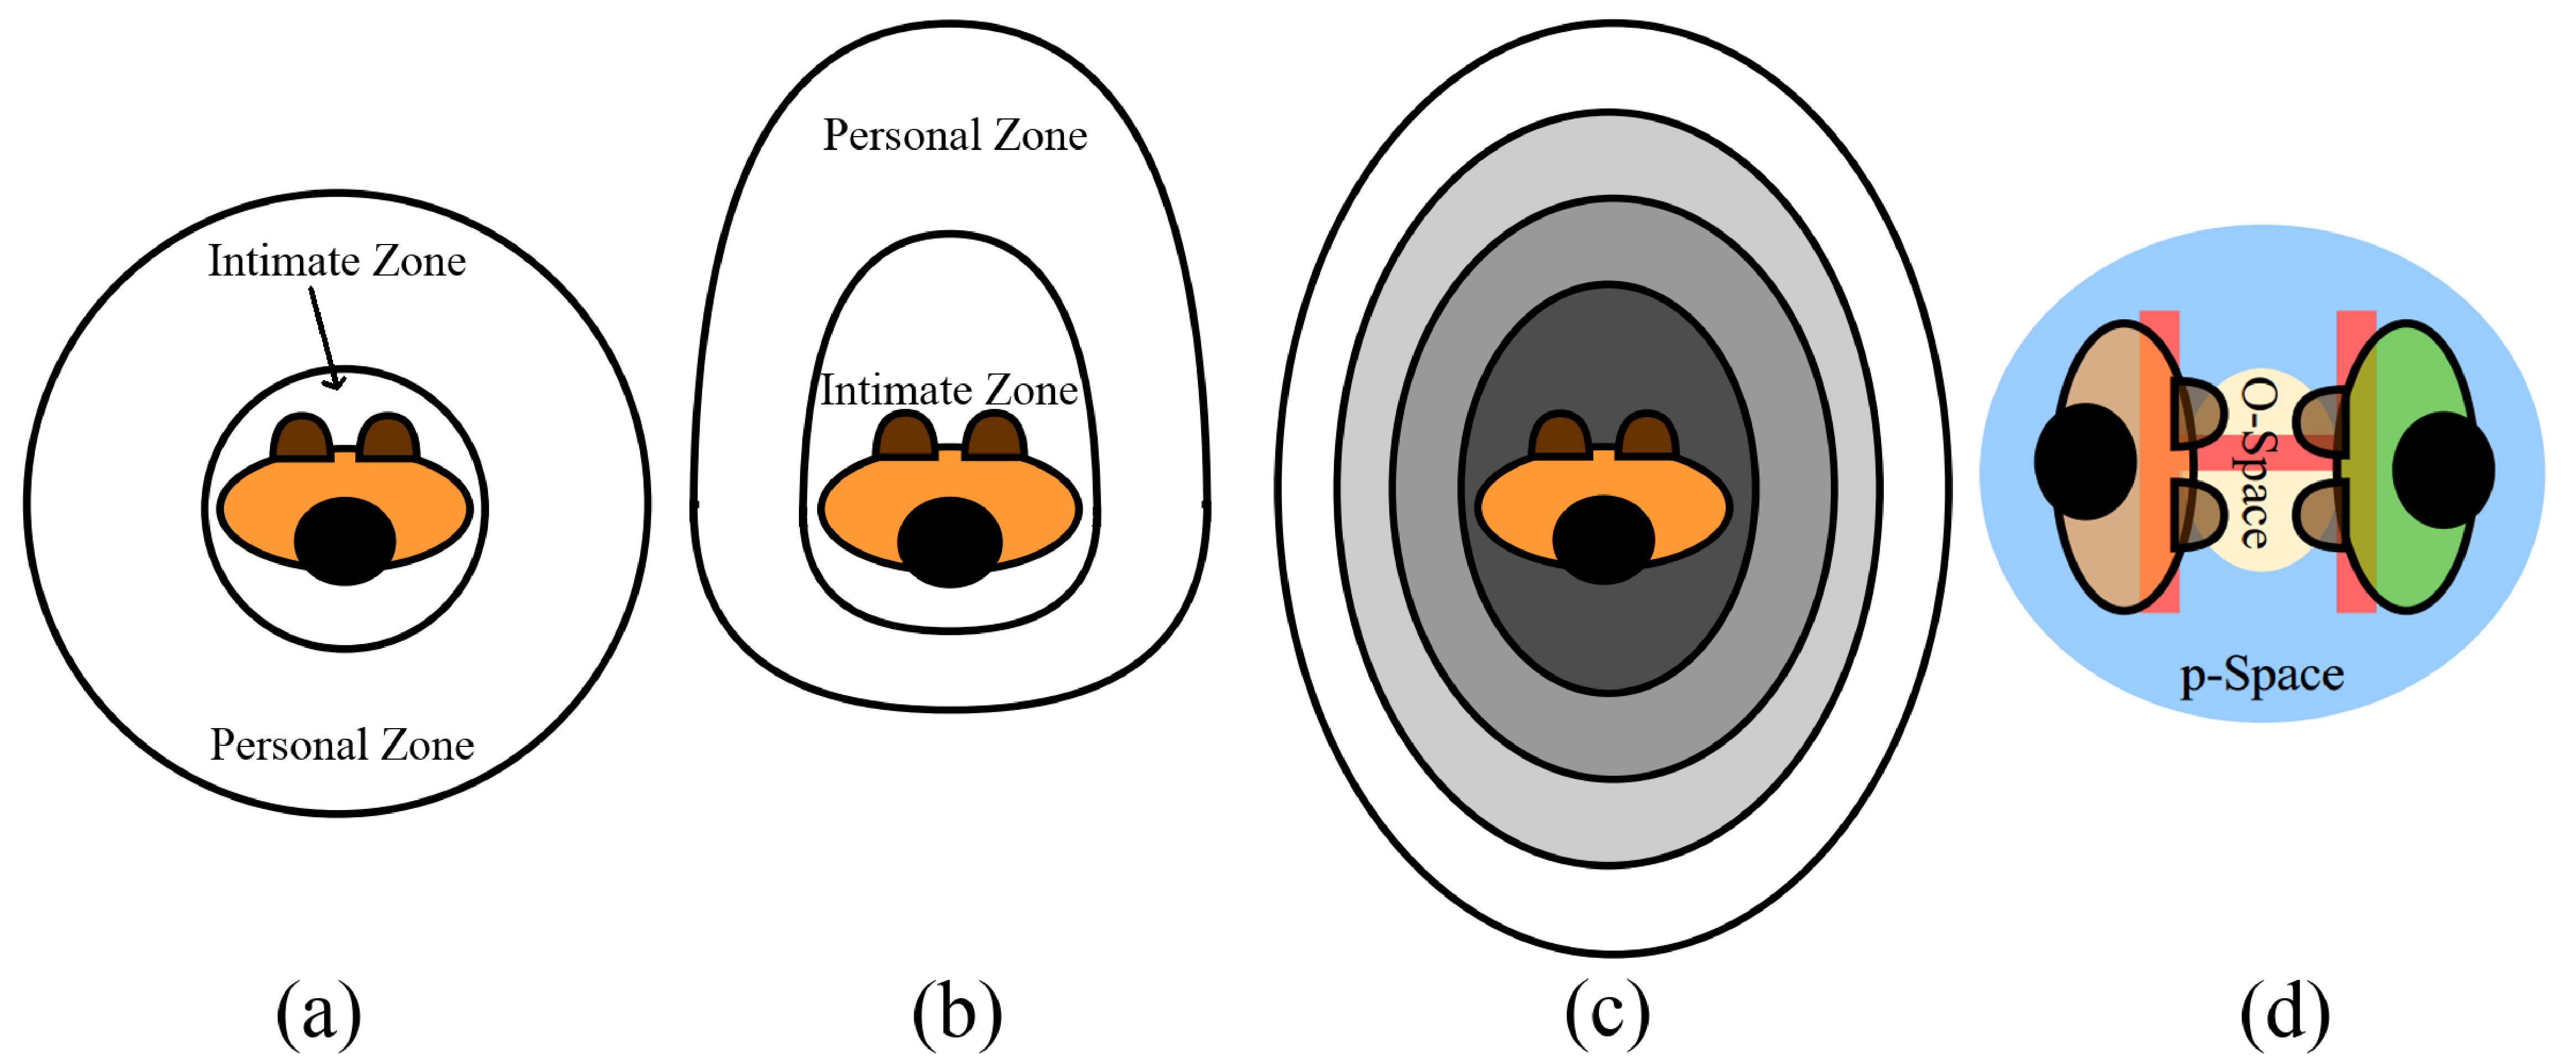
\includegraphics[width=0.95\columnwidth]{images/proxemics.eps}
    \caption{Zones and Spaces in Human and Group Modelling.}
    \label{fig:proxemics}
\end{figure}
For modelling humans, proxemics theory~\cite{hall_book_1966, mishra1983proxemics} provides some baselines that are common to most humans. Based on this, humans are designed as special obstacles with different zones around them. The very first modelling was done using concentric circles as shown in Fig.~\ref{fig:proxemics} (a) with four different zones~\cite{rios2015proxemics}, namely, 1) the public zone ($> 3.6m$), 2) the social zone ($> 1.2m$), 3) the personal zone ($> 0.45m$) and 4) the intimate zone ($\leq 0.45m$). These measures are not very strict and vary with age, culture, background etc. The robot can interact and enter the public and social zones while it is prohibited from entering the personal and intimate zones. Later different shapes are proposed for these zones \cite{rios2015proxemics} and the most commonly used one these days is the \textit{Egg} shape shown in Fig. \ref{fig:proxemics} (b) that makes the robot maintain a larger distance towards frontal side compared to the sides or back. This is specifically true in the case of moving humans, and some works \cite{kostavelis2016human} adapt the shape based on the estimated human velocity. As \acrshort{sfm} gained popularity in robotics, human is assumed to have a repulsive potential field in the shape of an ellipse that is monotonically decreasing with a peak at the centre. Fig. \ref{fig:proxemics} (c) shows this shape and the decaying potential field. The direction of this field is the direction of motion of the human. As research progressed, different concepts like Information Processing Space~\cite{kitazawa2010pedestrian} and Object Affordance Spaces were introduced into the human model. For groups, the concepts of \textit{o-space}, \textit{p-spaces}, and \textit{f-formations}~\cite{rios2015proxemics, kendon2010spacing} were introduced, which allowed the robot to avoid, join or leave a group of humans appropriately. An example of \textit{o-space} and \textit{p-space} with \textit{vis-a-vis} (or H) \textit{f-formation} is shown in Fig. \ref{fig:proxemics} (d). 

%%%%%%%%%%%%%%%Paper%%%%%%%%%%%
% https://link.springer.com/content/pdf/10.1007/978-3-642-04504-2.pdf
%%%%%%%%%%%%%%%%%%%%%%%%%%%%%%

It is necessary to predict the trajectory and motion of the human for the robot to act or react appropriately. As human detection and tracking is not the main focus of HAN, any off-the-shelf frameworks and systems can be used for this. After getting the necessary information about the humans' positions and velocities, a motion model is required to process these and predict the possible future trajectory. Thanks to the crowd navigation research, different methodologies like constant-velocity (or linear), \acrshort{orca}, \acrshort{sfm}, Social-LSTM~\cite{alahi2016social} etc., were developed, and these are usually employed for the motion models. The trajectory prediction is performed by forward simulating all the agents (humans and the robot) that are currently involved in HAN planning using their motion models (can be the same or different). Generally, the motion model has built-in collision avoidance strategies, and hence, the predicted trajectories are collision-free. However, when simplistic models are used (for example, linear), the trajectory prediction has to take care of collision avoidance as well.

%%%%%%%%%%%%%%Intention and Trajectory%%%%%%%%%%%%%
% Social Navigation Model based on Human Intention Analysis using Face Orientation
% You’ll Never Walk Alone: Modeling Social Behavior for Multi-target Tracking
% A Data-driven Framework for Proactive Intention-Aware Motion Planning of a Robot in a Human Environment
% A Review on Intention-aware and Interaction-aware Trajectory Prediction for Autonomous Vehicles
%%%%%%%%%%%%%%%%%%%%%%%%%%%%%%%%%%%%%%%
Human intention prediction is necessary to understand what humans might do in the future and take corrective actions. The meaning of intention may not be very clear as one can use it to refer to many things, like whether the human is going to cross the sidewalk or not \cite{kohler2012early}, which direction the human will move or turn next~\cite{peddi2020data}, whether the human is willing to interact or not~\cite{ratsamee2013social} and many others. Although intention prediction will greatly benefit HAN, it is not very easy to predict and generalise. The recent advancements in machine learning and computer vision provided tools that can be used to predict intentions, and some works \cite{peddi2020data, ratsamee2013social} have already integrated it into HAN.

%%%%%%%%%%%%Paper : Goal Prediction %%%%%%%%%%%%
% https://dendorferpatrick.github.io/GoalGAN/
% https://upcommons.upc.edu/bitstream/handle/2117/26703/1462-Bayesian-Human-Motion-Intentionality-Prediction-in-Urban-Environments.pdf;jsessionid=5DC717935D7D9E75A0A0167020803AAD?sequence=1
%%%%%%%%%%%%%%%%%%%%%%%%%%%%%%%%%%%%%%%%%%%%%%%%%

\subsubsection{Robot Planning and Decision Making}
In the early stages, HAN planning was done by adding the proxemic zones around the humans and then planning a path that avoids intrusions into the personal and intimate zones. This mostly involved grid search (like A*) or potential field based path planning with simple controllers that tracked the path. In most of these settings, the humans and the groups were static while the robot navigates around them. With progress in dynamic obstacle avoidance, different strategies evolved for HAN, like continuous re-planning of the path with updated proxemic zones \cite{truong2014dynamic} and temporal planning \cite{kollmitz2015time}. However, scalability is an issue with such global planning strategies, which consider the entire 2D map and all possible states to re-plan or update the path. On the other hand, as discussed previously, trajectory planning was mostly local and used only a small portion of the map and states. This offered a better alternative for doing temporal or reactive planning in HAN, and consequently, a lot of work today focuses on complex trajectory planning using simple path planning. As mentioned previously, the trajectory planning problem always involves some kind of optimization (minimization or maximization), and naturally, any kind of optimization technique could be employed to solve this problem. The `\textit{human awareness}' is included in the robot's motion (or trajectory) through the constraints of optimization, and sometimes they are referred to as `social or human-aware constraints'. Some commonly used optimization techniques in HAN include \acrshort{mpc} \cite{rosmann2021online}, Pareto-optimality \cite{forer2018socially}, graph optimization \cite{rosmann2013efficient} etc. There are other ways as well in which this problem was addressed, and some popular approaches are \acrshort{sfm}, velocity-obstacle based approaches (\acrshort{orca}, \acrshort{rvo} etc.), sampling based approaches like \acrshort{dwa} or \acrshort{rrt} and \acrshort{rl} based methodologies like \acrshort{cadrl}, \acrshort{sacadrl} etc.  

Trajectory planning in HAN should do more than simple collision avoidance with humans and obstacles. Since it is highly dependent on the context, it should best serve the task in the context rather than just avoiding discomfort. Therefore, the system has to be tuned to make the robot's motion legible and the interactions possible. One way to make robot's motion legible is through intention show using velocity or path modulation~\cite{kruse2014evaluating, lichtenthaler2013towards}, signals~\cite{may2015show} or visual projections~\cite{shrestha2018communicating}. All these have to be done while considering and following the social norms in the context. Some norms like `passing on right (or left)' could be employed using costmaps \cite{lu2013towards}, but some complex norms like waiting or advancing at a doorway to avoid blocking or giving way (moving to a side) for a human in a hurry require situation analysis and decision-making~\cite{zender2007human, granata2012framework, feil2011people, hayashi2012friendly} capabilities. Therefore, some of these works employ state machines that switch between behaviours, such as navigating in a crowd~\cite{dugas2020ian}, approaching a human~\cite{hayashi2012friendly}, following a human~\cite{zender2007human}, standing in line etc., after analysing the situation. Some other recent works use~\acrshort{pomdp}~\cite{qian2013decision} or deep learning~\cite{banisetty2020deep} based approaches to include the decision-making capabilities and modality switching into HAN.

In \acrshort{hri}, if the robot needs to communicate something or interact with a human, it needs to estimate `where' and `when' it should approach or meet the human and `how' it should plan its trajectory to be legible to all the humans in the environment (or context). Such things are usually addressed using Inverse Reinforcement Learning \cite{ramirez2016robots} or potential fields \cite{hansen2009adaptive}. Unlike the in-place communication that occurs in most \acrshort{hri} tasks, HAN planning has to communicate (through voice or gestures) during navigation to negotiate or prevent the occurrence of the \acrshort{frp}. This is usually done by maintaining a knowledge base and a model \cite{dugas2020ian} that decides `what' and `when' to communicate. This again emphasises the need for decision-making in HAN.

\section{Background and Our Approach}
In this section, we provide details on the mathematical modelling and the background that is necessary to understand our approach to HAN planning. We present the~\acrshort{teb} formulation and its hypergraph modelling, followed by the formulation of \acrshort{hateb} and the modelling of social constraints. Following this, the application of the joint-action principles of \acrshort{hri} to HAN is presented. Finally, we discuss our ideology while developing a HAN system and briefly describe the approach.

\subsection{Timed Elastic Band for Trajectory Planning}
\acrfull{teb} for trajectory planning was proposed by R{\"o}smann et al.~\cite{rosmann2013efficient} and is available as one of the local planners\footnote{\url{http://wiki.ros.org/teb_local_planner}} in \acrshort{ros}. This approach uses hypergraph representation to build the timed elastic band and then optimizes the graph to get the optimal command velocity. We briefly provide the mathematical details of this framework here.

\subsubsection{TEB Formulation}
The robot's trajectory in 2D navigation can be represented as a sequence of $n$ poses, $p_i = (x_i, y_i, \theta_i) \in \mathbb{R}^2 \times S^1$  and with a set of $n-1$ time intervals, $\delta t_i \in \mathbb{R}^+$ between two consecutive poses. Classically, in an elastic band \cite{quinlan1993elastic} approach, only the poses were considered along with the kinematic model of the robot, and therefore, the obtained trajectory may not satisfy the dynamic constraints of the robot. On the other hand, \acrshort{teb} considers both poses and time intervals and hence, the resultant trajectory is both kinematically and dynamically feasible. Let the sequence of poses, $\{p_i\}$, and the time intervals $\{\delta t_i\}$ be represented by:
\begin{equation*}
    \begin{aligned}
      P & = \{p_i\}_{i=0...n} \quad n \in \mathbb{N} \\
      \tau & = \{\delta t_i\}_{i=0..n-1} 
    \end{aligned}
\end{equation*}

Using these sequences, $P$ and $\tau$, \acrshort{teb} is defined as a tuple:
\begin{equation}
    B := (P,\tau)
\end{equation}

\acrshort{teb} is then optimized using a weighted multi-objective optimization to obtain the optimal poses and time intervals in real-time:
\begin{equation}
    f(B) = \sum_k \alpha_kf_k(B)
\end{equation}
\begin{equation}
    B^* = \argmin_B f(B)
\end{equation}
where $f(B)$ is the objective function and $B^*$ denotes the optimized \acrshort{teb}. The objective function $f(B)$ is a weighted (by $\alpha_k$) sum of different components $f_k(B)$ that represent different kinodynamic constraints. The constraints are formulated as objectives in terms of a piecewise continuous, differential cost function that penalises the violation of a constraint \cite{rosmann2013efficient}.

\subsubsection{Hypergraphs and TEB Hypergraph}
A hypergraph is a generalised graph with hyperedges \cite{bretto2013hypergraph} that can connect any number of vertices (or nodes), unlike a normal graph where an edge connects only two vertices.
\begin{figure}[!h]
    \centering
    \begin{subfigure}[t]{0.45\columnwidth}
        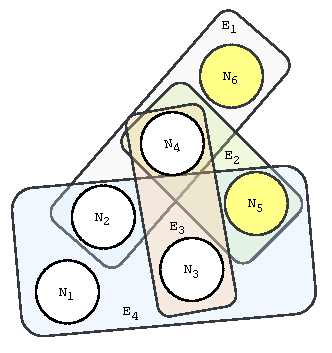
\includegraphics[width=0.9\textwidth]{images/hypergraph.pdf}
    \caption{A general hypergraph}
    \end{subfigure}
     \begin{subfigure}[t]{0.45\columnwidth}
        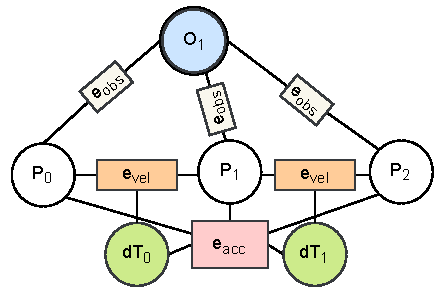
\includegraphics[width=\textwidth]{images/hypergraph_teb.pdf}
    \caption{Hypergraph used in TEB}
    \end{subfigure}
    \caption{HyperGraph}
    \label{fig:hypergraph}
\end{figure}
Mathematically, if $H$ is a hypergraph and $V$ is the set of vertices, and $E$ is the set of hyperedges, then
\begin{equation}
    H = (V, E) \implies E = \{e_i \mid e_i \subseteq V\} \forall i \in I
\end{equation}
where $I$ is a finite set of indices. An example of a hypergraph is presented in Fig. \ref{fig:hypergraph} (a) with six vertices and four edges. Hypergraphs can contain different kinds of vertices and edges. In Fig. \ref{fig:hypergraph} (a) each edge is of a different kind (different colours), and there are two different types of vertices (yellow and white). 

Using hyperedges, any mathematical relationship between any of the vertices can be defined, and this plays an important role in the HAN system proposed in this thesis. Therefore hyperedges can naturally be employed to model the kinodynamic constraints of the robot, and so \acrshort{teb} is modelled using a hypergraph. The vertices of this hypergraph are the poses and the time differences, while the hyperedges represent different constraints or relations between these vertices. A small part of this hypergraph is presented in Fig. \ref{fig:hypergraph} (b), containing five vertices (three poses and two time differences), and shows the velocity, acceleration and obstacle edges. The obstacle is shown in blue with concentric circles. From this figure, it can be seen that the constraints are mostly local, as they depend only on a few consecutive configurations. It is also the case for the majority of the components in the objective function, $f(B)$, of \acrshort{teb}, and hence, the \acrshort{teb} hypergraph has a sparse system matrix. Therefore, this hypergraph can be optimized online and in real time. \acrshort{teb} is optimized using an open-source graph optimization framework, g2o, which we present next. 

\subsubsection{g2o Optimization}
g2o (or General Graph Optimization) \cite{grisetti2011g2o} is an optimization framework developed for solving graph-based nonlinear error function. It offers solutions to the problems with the following structure:
\begin{equation}
\label{eq_optim}
  \mathbf{F(x)} = \sum_{k=\langle i,j \rangle} \mathbf{e}_k(\mathbf{x}_i, \mathbf{x}_j, \mathbf{z}_{ij})^T \mathbf{\Omega}_k\mathbf{e}_k(\mathbf{x}_i, \mathbf{x}_j, \mathbf{z}_{ij}) 
\end{equation}
\begin{equation}
    \mathbf{x}^* = \argmin_\mathbf{x} \mathbf{F(x)}
\end{equation}
where $\mathbf{x}$ represents the parameters to be optimized, $\mathbf{x}_i$, $\mathbf{x}_j$ are the block parameters and $\mathbf{z}_{ij}$ denotes the constraint between them. $\mathbf{\Omega}_k$ denotes the information matrix between the constraints and $\mathbf{e}_k(\mathbf{x}_i, \mathbf{x}_j, \mathbf{z}_{ij})$ is the error vector between the parameters and the constraint. The optimized set of parameters is represented by $\mathbf{x}^*$. Note that, the part inside the summation in Eq. \eqref{eq_optim} becomes $\Omega_k e_k^2$ if the error is scalar. In case of \acrshort{teb} \cite{rosmann2013efficient}, the objective function, $f(B)$ takes the above form where $B$ is the set of parameters to be optimized, $\mathbf{x}$, $\alpha_k = \Omega_k$, $e_k = \sqrt{f_k}$ and $\mathbf{x}_i = (p_i, \delta t_i)$. g2o uses the Levenberg-Marquardt method to optimize the objective function numerically and offers two Cholesky decomposition solvers, CHOLMOD and CSparse, to solve it efficiently.

\subsection{Human-Aware Timed Elastic Bands for Proactive Planning}
In this section, we present the idea of \acrfull{hateb}, proposed by Khambhaita and Alami~\cite{khambhaita2017viewing} that lays the basis for this thesis. We briefly discuss how the objective function and hypergraph are modified to include human-aware constraints in robot navigation. 

\subsubsection{HATEB Formulation and Hypergraph}
The idea of \acrshort{hateb} is to add elastic bands to all the humans in the robot's vicinity in addition to the robot and jointly optimize the robot and the human trajectories under kinodynamic and human-aware (or social) constraints. This gives rise to a multivariate multi-objective optimization problem to solve, and the same weighted sum approach proposed in \acrshort{teb} is used for \acrshort{hateb} as well. Therefore, if the robot's band is represented by $B_r$ and the human bands by $\{B_{h_k}\}_{k=0}^n$ when $n (\in \mathbb{N})$ humans are present in the vicinity, the new objective function to solve is,
\begin{equation}
    \label{hateb_eq}
    f(B_r, B_{h_0}...B_{h_n}) = \underbrace{\sum_{i}\alpha_i f_i(B_r)}_{F_R} + \sum_k \left (\underbrace{\sum_{j}\alpha_j f_j(B_{h_k})}_{F_H} + \underbrace{\sum_l \alpha_l f_l(B_r, B_{h_k})}_{F_S} \right )
\end{equation}
\begin{equation}
    B_r^*, B_{h_0}^*...B_{h_n}^* = \argmin_{B_r, B_{h_0}...B_{h_n}} f(B_r, B_{h_0}...B_{h_n})
\end{equation}
where $B_r^*, \{B_{h_k}^*\}_{k=0}^n$ are optimized trajectories for the robot and the humans respectively. The initial paths of humans for this optimization is obtained from the human path prediction module of the system.
\begin{figure}[!h]
    \centering
    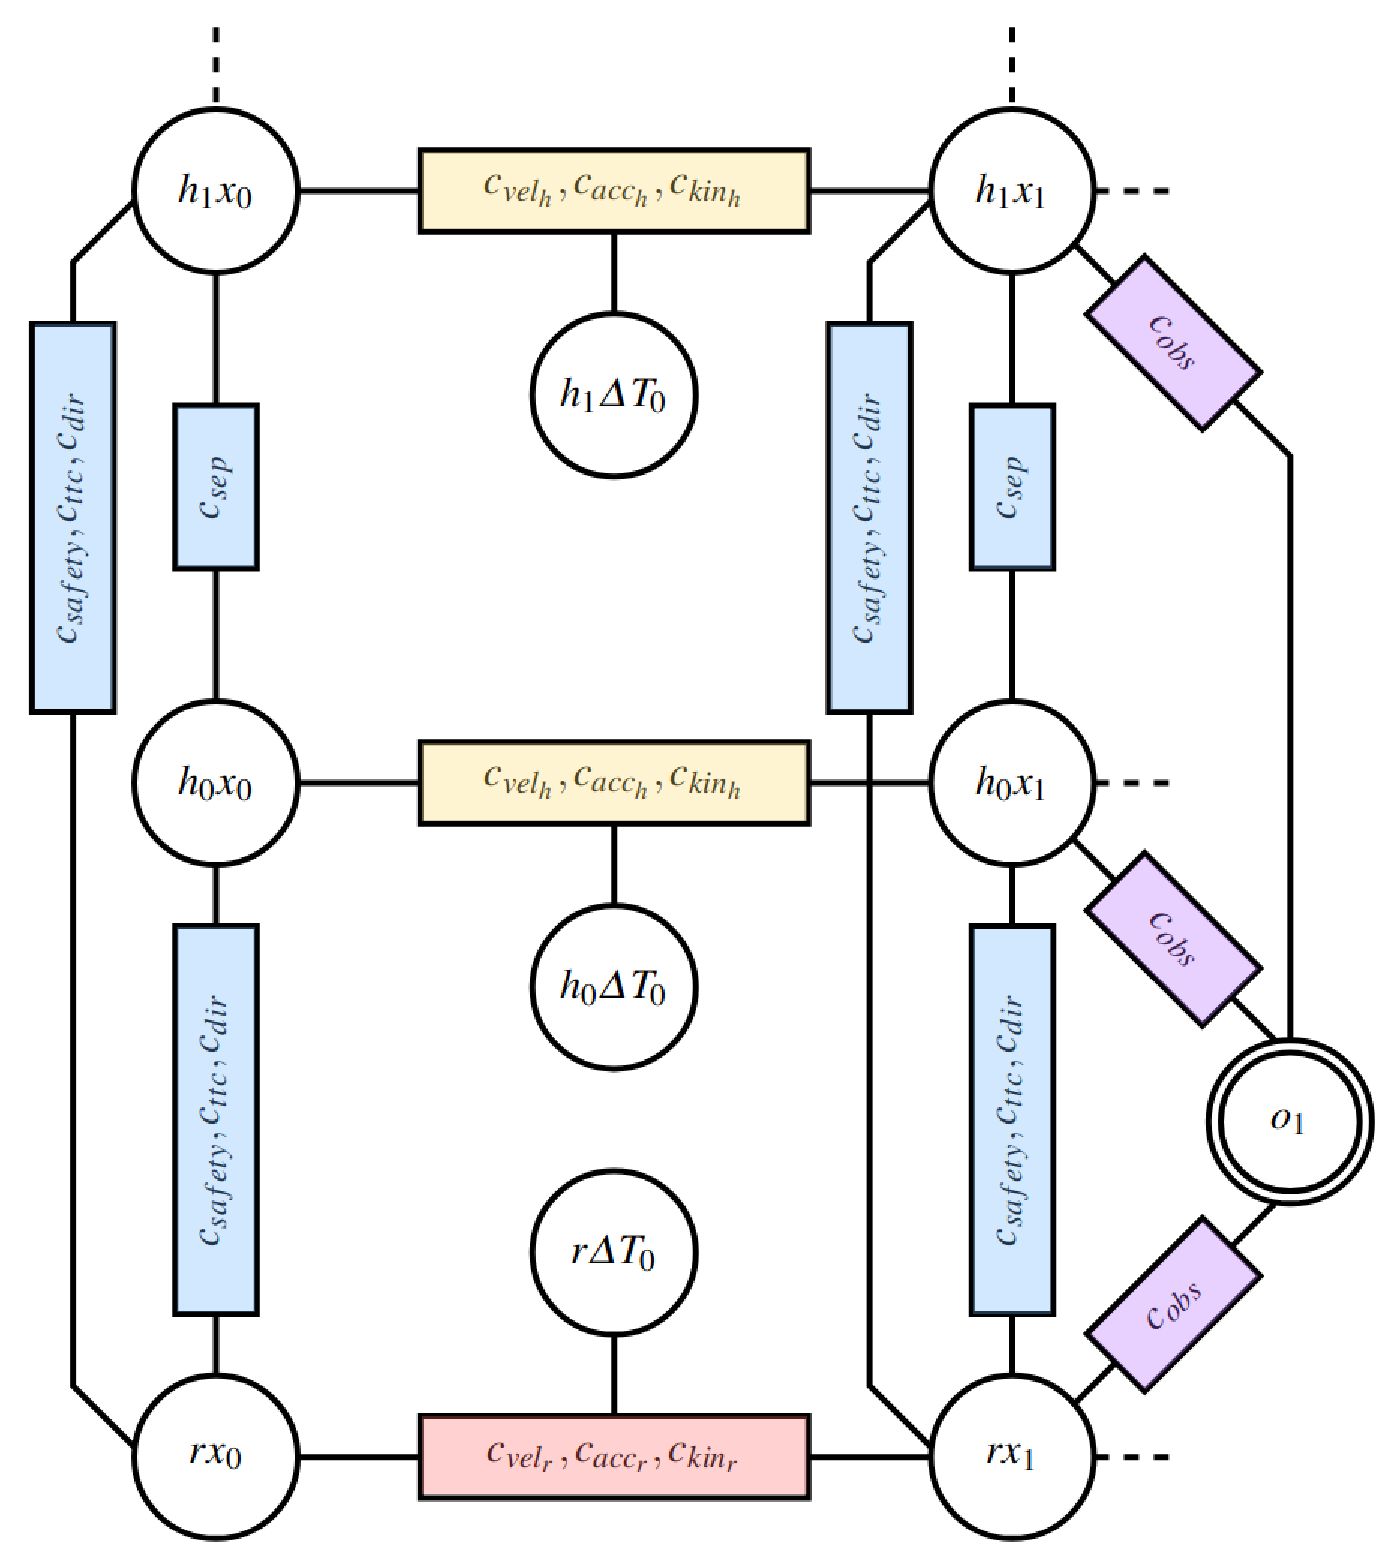
\includegraphics[width=0.65\columnwidth]{images/hateb_new.pdf}
    \caption{The updated hypergraph of HATEB~\cite{khambhaita2017viewing}. There are 3 bands, one for the robot and the other two for humans. The kinodynamic constraints are shown as horizontal edges (yellow, red), social constraints are shown as vertical edges (blue), and the obstacle avoidance constraints are shown as diagonal edges (purple).}
    \label{fig:hateb_hypergraph}
\end{figure}

In Eq.~\ref{hateb_eq}, $F_R$ and $F_H$ represent the objective functions for the robot and human trajectories, whereas $F_S$ denotes the objective for human-robot social constraints. All these constraints are represented as hyperedges of an updated hypergraph, and a small part of this hypergraph is shown in Fig. \ref{fig:hateb_hypergraph}. The social constraints between human-robot and human-human are highlighted in blue, while the kinodynamic constraints of the robot and humans are highlighted in red and yellow, respectively. Finally, the obstacle constraints are shown in purple. Even though the system matrix is still sparse, it is denser than before, and as we keep adding bands for humans, the density grows, and the trajectories cannot be obtained in real-time. 

\subsubsection{Proactive Planning and Social Constraints}
The joint optimization produces the robot trajectory that obeys the social norms implemented in $F_S$. Further, the combined human-robot trajectory planning makes the robot proactively estimate humans' plans and quickly adapt its trajectory before it is too late. We call this idea of adding double-sided (robot side, human side) bands as `{\textit{Dual Band}}' throughout this thesis. This approach always elicits solutions (provided they exist) for all agents, which can solve the navigation scenario at hand if every agent follows its trajectory. 
Using the above architecture, three social constraints are defined, 1) \textit{Human-Robot Safety}, which takes care of human safety and proxemics, 2) \textit{\acrfull{ttc}}, which adds early intention show to the robot's trajectory and 3) \textit{Directional}, that tries to establish a trade-off between slowing down and changing the path. In \acrshort{hateb}, the objective function for safety clearance from obstacles is also updated to make the robot move towards obstacles rather than humans in confined scenarios. All these constraints are added to the objective function as piecewise continuous and differential error functions, like in \acrshort{teb}. We believe that this architecture is better suited to solve the HAN problem than the reactive approaches, especially in intricate indoor scenarios.

\subsection{Principles of Joint-Action in Human-Aware Navigation}
As mentioned previously, HAN can be seen as a part of \acrshort{hri} and therefore, we believe that it should possess some of the properties of \acrshort{hri}. Specifically, during the development of this thesis, the principles of joint-action \cite{curioni2019joint} in \acrshort{hri} were applied to HAN. These principles include: sharing a common perspective, coordinating, predicting others' contributions and communicating. In terms of human-aware robot navigation, these can be seen as:
%%%%%%%%%%%Paper%%%%%%%%%%%%%%%%%
% https://www.researchgate.net/publication/328209329_Joint_Action_in_Humans_A_Model_for_Human-Robot_Interaction
%%%%%%%%%%%Paper%%%%%%%%%%%%%%%%%
\begin{itemize}[leftmargin=*]
    \item \textit{Share a common perspective}: The robot should know the social norms and expectations of a human in a given environment. For example, moving on the right, avoiding collisions with humans and other objects etc.
    \item \textit{Coordination}: The robot and human should coordinate and cooperate with each other to reach their navigation goals. For example, the robot should give way for the human to pass in a door crossing scenario instead of blocking.
    \item \textit{Predict others' contribution}: The robot should predict humans' motion (trajectory) and/or intentions to know how much the human is willing to contribute to the navigation task. For example, in a corridor, the robot facing a human can either continue with or change its path depending on whether the human is willing to change his/her path or not. 
    \item \textit{Communication}: The robot should be able to communicate to humans what action it is going to take or sometimes take permission or inform humans before taking an action. Communication in HAN can be split into two types, 1) Communicating navigation intention (for example, signals) and 2) Communication through speech or video to negotiate in a complex scenario.
\end{itemize}
These principles impose more restrictions on the robot's trajectory and require the inclusion of decision-making capabilities into robot navigation planning. This makes HAN a complicated problem to solve in the motion planning paradigm. 

\subsection{Our Approach and Contribution}
One of the noted limitations with \textit{Dual Band} approach is that it assumes that humans are always cooperative agents and will not cause any deadlock situations. So it always proposes solutions with the assumption that the human will be moving, which might not be the case. When the human stops moving or behave unconventionally, the robot gets stuck without moving or oscillates without making any progress towards the goal. Therefore, we introduce situation assessment over proactive planning as shown in Fig. \ref{fig:full_contrib}. This situation analysis is local and happens at the trajectory planning level. 
\begin{figure}[h!]
    \centering
    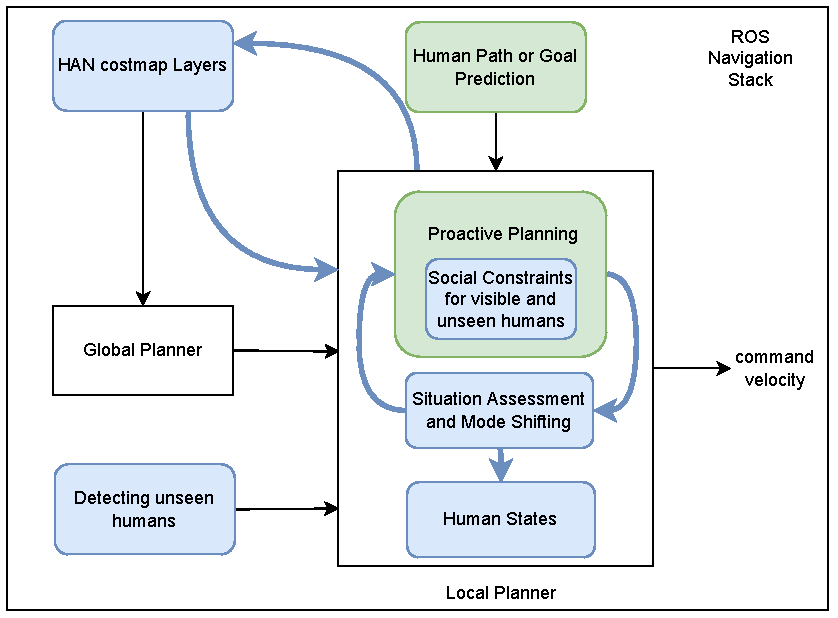
\includegraphics[width=0.9\columnwidth]{images/contrib_new.pdf}    \caption{The situation assessment module is combined with proactive planning inside the local planner. The system can use any existing global planner.}
    \label{fig:full_contrib}
\end{figure}
After analysing a situation and determining if it's a deadlock or any other uncomfortable setting, we have to find a way to mitigate it. In this thesis, we do this by shifting between different navigation modalities. The blue arrows in Fig. \ref{fig:full_contrib} represent how proactive planning, situation assessment and mode shifting are interlinked with each other. The integration of situation analysis into trajectory planning and the process of mode shifting are presented in detail in the subsequent chapters.

The crux of this thesis is finding and mitigating the uncomfortable human-robot interactions in HAN. Note that this includes the humans in view and the humans the robot has not seen yet. The main contributions of this thesis in developing a human-aware \acrshort{ros} navigation stack are shown in coloured boxes in Fig. \ref{fig:full_contrib}. The ones in blue colour are the new contributions, while the ones in green represent modifications over the previous work. The blue arrows stand for the new connections we have made in our proposed HAN. Proactive planning has been significantly improved by proposing new human-robot social constraints for both visible and unseen humans. The updated path prediction module with new goal prediction methodologies further improves proactive planning, and hence, better navigation behaviours can be obtained. The new HAN costmap layers are proposed to specifically address the global planning around static humans. Yet, these layers update based on the states of humans (blue arrows) given by the local planner and play a role in trajectory planning as well. While analysing a situation, the state of the human (static, moving, stopped etc.) is necessary, and hence, situation assessment modules maintain a list of states for the humans it has encountered during its navigation. The choice of modality is based on the state of the human as well as the situation. The idea of mitigating collisions with unseen humans is quite new in the case of HAN and makes the robot ready to face any kind of situation when combined with the multi-context HAN system proposed in this thesis. We believe that the idea of mode shifting within local planning is significantly new and can be seen as a major contribution as well.



